% Created 2019-11-06 Wed 19:27
% Intended LaTeX compiler: pdflatex
\documentclass[11pt]{article}
\usepackage[utf8]{inputenc}
\usepackage[T1]{fontenc}
\usepackage{graphicx}
\usepackage{grffile}
\usepackage{longtable}
\usepackage{wrapfig}
\usepackage{rotating}
\usepackage[normalem]{ulem}
\usepackage{amsmath}
\usepackage{textcomp}
\usepackage{amssymb}
\usepackage{capt-of}
\usepackage{hyperref}
\author{Nick Merrill}
\date{\today}
\title{III: Metrics and radar plots}
\hypersetup{
 pdfauthor={Nick Merrill},
 pdftitle={III: Metrics and radar plots},
 pdfkeywords={},
 pdfsubject={},
 pdfcreator={Emacs 25.2.2 (Org mode 9.1.14)}, 
 pdflang={English}}
\begin{document}

\maketitle
I've collected metrics for all of 2019, for all of the data sources in our
dataset. There may be an issue with our layer 3 (internet interference) data,
but as we diagnose, I thought it would be a fair time to introduce the
particulars of the metrics and share some preliminary radar charts (with the
caveat that data may change).

We may be all on the same page with metrics, but often, the devil is in the
details. It's worth going through each layer's metrics and discussing their
particulars.

\section{One metric per layer}
\label{sec:org7813c1c}
\subsection{Layer 2: IPv6 adoption}
\label{sec:org5ef244e}

As a proxy for interlink layer (layer 2) fragmentation, we use \href{https://www.google.com/intl/en/ipv6/statistics.html\#tab=per-country-ipv6-adoption}{Google's
per-country IPv6 adoption statistics}, which Google collects from all Google
services and analytics users. I suspected that they would radically
under-estimate adoption in China, where Google is blocked, but surprisingly,
Google's statistic \href{http://www.xinhuanet.com/english/2019-03/14/c\_137895292.htm}{roughly matches the one given by state-run Chinese media}.

\subsection{Layer 3: Network interference events}
\label{sec:org7a8d8ae}

To measure transport layer (layer 3) fragmentation, we use data collected by the
\href{https://ooni.org/}{Open Observatory of Network Interference} (OONI). OONI requires volunteers to
install a plugin, which periodically performs tests to measure circumvention on
the transport layer. These include mostly state-launched attacks (such as DNS
manipulation or traffic filtering), but may also include private-sector
manipulation, such as throttling streaming traffic.

Since different countries produce radically different numbers of reports per
year, we compute a "rate" of anomalous observations per all reports generated.

\subsection{Layer 4: Website ranking locality}
\label{sec:org7776fba}

We use the \href{https://www.alexa.com/topsites}{Alexa rankings} to determine the 50 most popular websites in every
country (by traffic). We then compare each country's most popular websites to
the worldwide most popular websites, using \href{https://en.wikipedia.org/wiki/Levenshtein\_distance}{Levenshtein distance} to compute the
edit distance between the two lists. This leaves us with a metric expressing how
much each country's web browsing habits differs from the global rankings. \footnote{To pump the intuition here\ldots{} At the bottom of these rankings (most
country-specific), we have China; at the top (most similar to the global
rankings), we have Luxembourg.} 


\subsection{Layer 5: Data locality laws}
\label{sec:orgdb81ead}

Right now, I count one type of data locality law: whether a given country
restricts the cross-border flow of data (any type). We code this as a binary
variable. 

One clear issue with this metric: it's binary, which removes some subtlety from
the radar chart. I have brainstormed different ways to make this metric a bit
more (numerically) nuanced in the future (see \ref{orgc398867}).

\section{Visualizing the metrics: Radar charts}
\label{sec:org43469fa}

How do we visualize these metrics? Right now, our strategy is to produce a
"radar" (or "spiderweb") plot. The radar plot describes a given country's spread
across the four metrics we currently measure. By visually comparing these radar
plots, we can establish rough "profiles" for countries. \footnote{For ease of display in a radar plot, we transform all data to be between
0 and 1, and assure all continuous variables are roughly normally distributed.
Setting aside our binary variable (layer 5), both Layer 2 and Layer 4's metrics

are (rougly) normally distributed. Layer 3's metric, on the other hand, is
roughly a power law distribution (i.e., a few countries have 10-100x the rate of
network inteference as the majority). We "view" these data on a logarithmic
scale in the radar plot, (I confirmed that the log-scale data are roughly
normal).}


\begin{center}
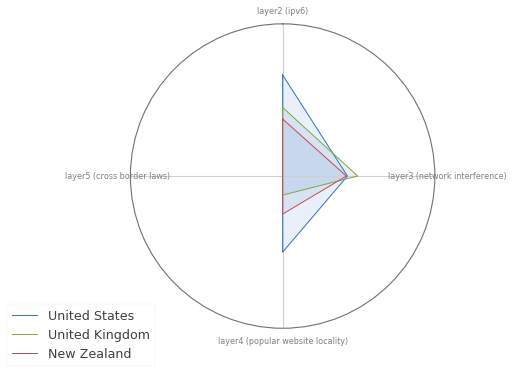
\includegraphics[width=.9\linewidth]{./figures/us-uk-nz.png}
\end{center}

Here's an example. It compares the US, UK and New Zealand. This radar chart
shows us that the UK and New Zealand are similar, but the United States shows
more fragmentation on layers 2 and 3. However, all three countries have no
restrictions on cross-border data flow, and they all have about the same amount
of network interference. \textbf{NOTE}: /Data may change slightly here as we sanity
check our preprocessing---layer 3 data in particularespecially /.


\begin{center}
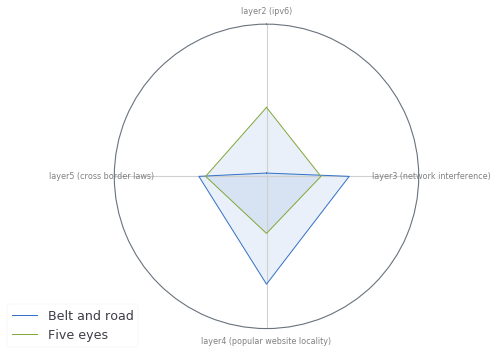
\includegraphics[width=.9\linewidth]{./figures/belt-and-road.png}
\end{center}

We can also average multiple countries' metrics together to create \emph{blocks}.
Here's an example comparing Five Eyes countries with Belt and Road countries.
Overall, Belt \& Road countries have higher website locality (perhaps as a result
of censorship), higher rates of network interference, and very low adoption of
IPv6. (They have slightly higher rates of having cross-border data transfer laws,
but it's not clear yet whether the difference is significant).

\section{Reflections}
\label{sec:org85bfbdd}

\subsection{Introducing variation into Layer 5}
\label{sec:org4730c62}
\label{orgc398867}

This binary variable doesn't give us enough variation. As much as I'm loathe to
"generate quantification," one possibility is to bucket data-related laws by
domain (cross-border data flows, privacy, data sovereignty), code them as binaries
per category, and sum them. This will produce an aggregate score in which all
data-related laws are equally weighted. What do folks think about this approach?
See Appendix \ref{org827f471} for the types of data laws we coded over the summer.


Cons:
\begin{itemize}
\item This may get us in trouble with sticklers, who will argue that not all data
laws are equally consequential.
\end{itemize}

Pros:
\begin{itemize}
\item It will certainly introduce variation into our metric, and hopefully will
produce a normal (rather than bimodal) distribution among countries.
\end{itemize}

\subsection{Dealing with the European Union}
\label{sec:orgd46a40c}

For our layer 5 metric, the European Union (GDPR) is tricky here. GDPR does
restrict certain types of cross-border data flows. For now, I've counted all EU
member states as "yes," as the GDPR laws apply there. However, this law
restricts data flows \emph{out of the EU}, not (e.g.) between Belgium and
Netherlands. So having each country ``inherit'' the EU law may be misleading.

In the future, we may want to include EU \textbf{and} member states as separate, if
geographically overlapping entities for our analysis. Any thoughts on this would
be much appreciated.

\subsection{Layer 5: Are laws enforced?}
\label{sec:orge9e06a3}

Are the laws described in Layer 5 enforced? Our metric does not currently
capture this question. It could, but may require some bespoke input from people
"on the ground," which we are trying to avoid right now. I'm inclined to ignore
this for now, and add it to the ``think about later'' pile (a pile I am, for the
record, diligently collecting).

\section{Appendix}
\label{sec:org0c4318b}

\subsection{Data laws by type}
\label{sec:orgeacce21}
\label{org827f471}

\begin{itemize}
\item Online sales
\item Domain name (DNS) registration requirements
\item Export restrictions
\item Bandwidth, net neutrality
\item Lack of safe harbor for intermediary liability
\item Sanctions for non-compliance
\item Administrative requirements on data privacy
\item Data retention
\item Restrictions on cross-border data flows
\item Other restrictive practices related to business mobility
\item Quotas, Labour Market Tests, Limits of Stay
\item Other restrictive practices related to competition policy
\item Competition
\item Copyright
\item Patents
\item Screening of investment and acquisitions
\item Restrictions on ownership
\item Technology mandate
\item Preferential purchase schemes covering digital products and services
\item Discriminatory tax regime on online services
\item Discriminatory tax regime on digital goods and products
\item Antidumping, CVD \&amp; Safeguards
\item Applied tariffs on digital goods
\item Barriers to fulfillment
\item Product screening and testing requirements
\item Product safety certification (EMC/EMI, radio transmission)
\item Import restrictions
\item Censorship and filtering of web content
\item Notice and takedown requirement
\item Other
\item Personal rights to data privacy
\item Trade secrets
\item Other restrictive practices related to foreign investment
\item Restrictions on board of directors and managers
\item Taxation on data usage
\item Other restrictive practices related to IPR
\item Telecom network and base standards
\item Local Content Requeriments for commercial market
\item Requirement to surrender patents, source codes, trade secrets
\item Subsidies and favourable tax regime
\item Other restrictive practices related to content access
\item Encryption
\item Other restrictive practices related to standards
\item Discriminatory / disproportionate consumer protection
\item Other restrictive practices related to intermediary liability
\end{itemize}
\end{document}
